\subsection{Exploratory Data Analysis}
% \subsubsection{content}
    % unique voters
    By the end of 2017, there is a total number of 573 contests in the platform. To identify what kind of content that is more engaging (RQ2), first let us look at the amount of unique voters over the number of contests. Figure \ref{user_engagement_in_contests} displays a histogram and a boxplot of the number of contests and the number of unique voters that they have engaged. 
    
    \begin{figure}[h] 
        \begin{center}
            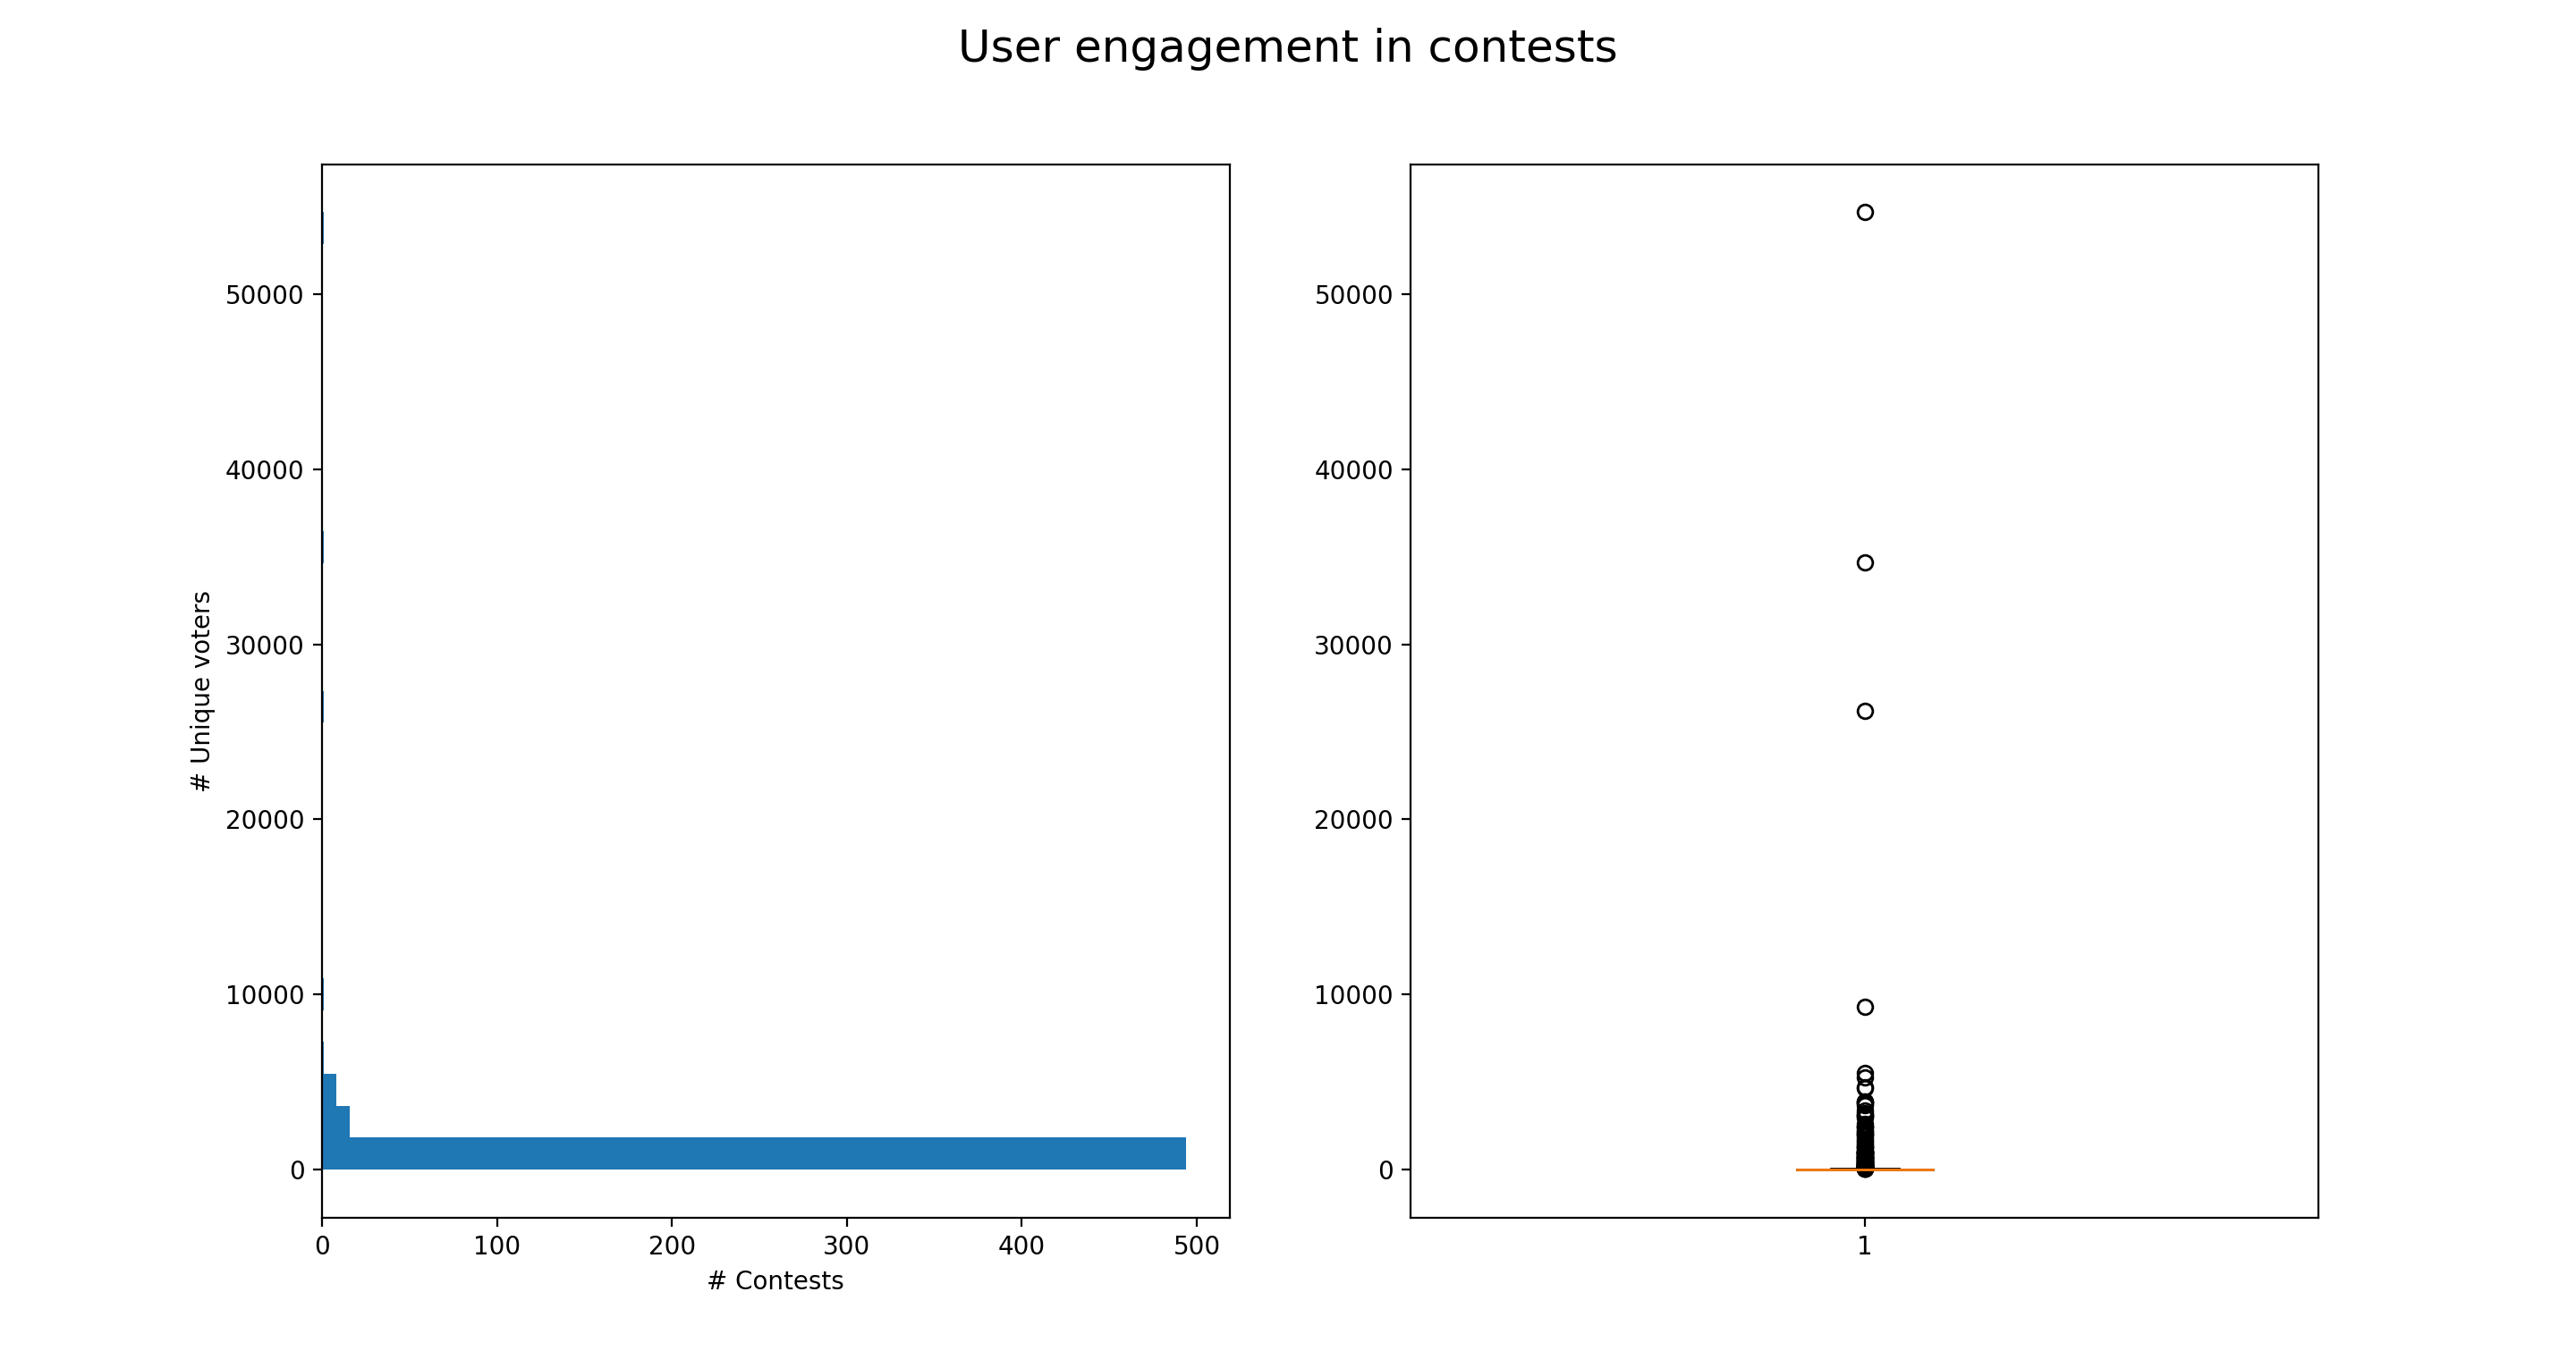
\includegraphics[width=0.8\textwidth]{Images/user_engagement_in_contests.png}
            \caption{The number of unique voters over contests.}
            \label{user_engagement_in_contests}
        \end{center}
    \end{figure}

    It can be easily seen that most of the contests engage very small amount of users, as the median of the unique voter count for all contests is 3. One of the reasons behind this is that the company did not establish a large user base yet. Therefore there are many users who created only one contest but never used the platform on the long run. Many of the contests serve only testing purposes, hence engage only a few users. Such records can create bias in the upcoming analyses, because their data does not represent realistic scenarios. For this reason, contests with less than $100$ unique voters are excluded in the remainder of the analysis, because such observations are not representative. For the remainder of the analyses, this filtered dataset is used.

    Figure \ref{user_engagement_in_contests-pruned} displays the same distribution for the filtered set of contests. In this figure contests with more voters are more apparent. The highest number of unique voters is close to $55 000$ in one of the contests, the mean value ($\mu = 455.43$) and the standard deviation ($\sigma = 3 017.51$). These numbers mean that there is a large variance in the amount of engaged users in contests. It cannot be clearly said which traits make a contest more attractive to users.
    
    The boxplot on the right side of the figure uses the $95$ percentile (around $5 200$ unique voters), above which the outliers can be seen. It can be also seen that the most of the contests engage $260-2 600$ unique voters (as described by the first and the third quartiles). There are $6$ large contests, from which the biggest have engaged $54 684$ voters. 

    \begin{figure}[h] 
        \begin{center}
            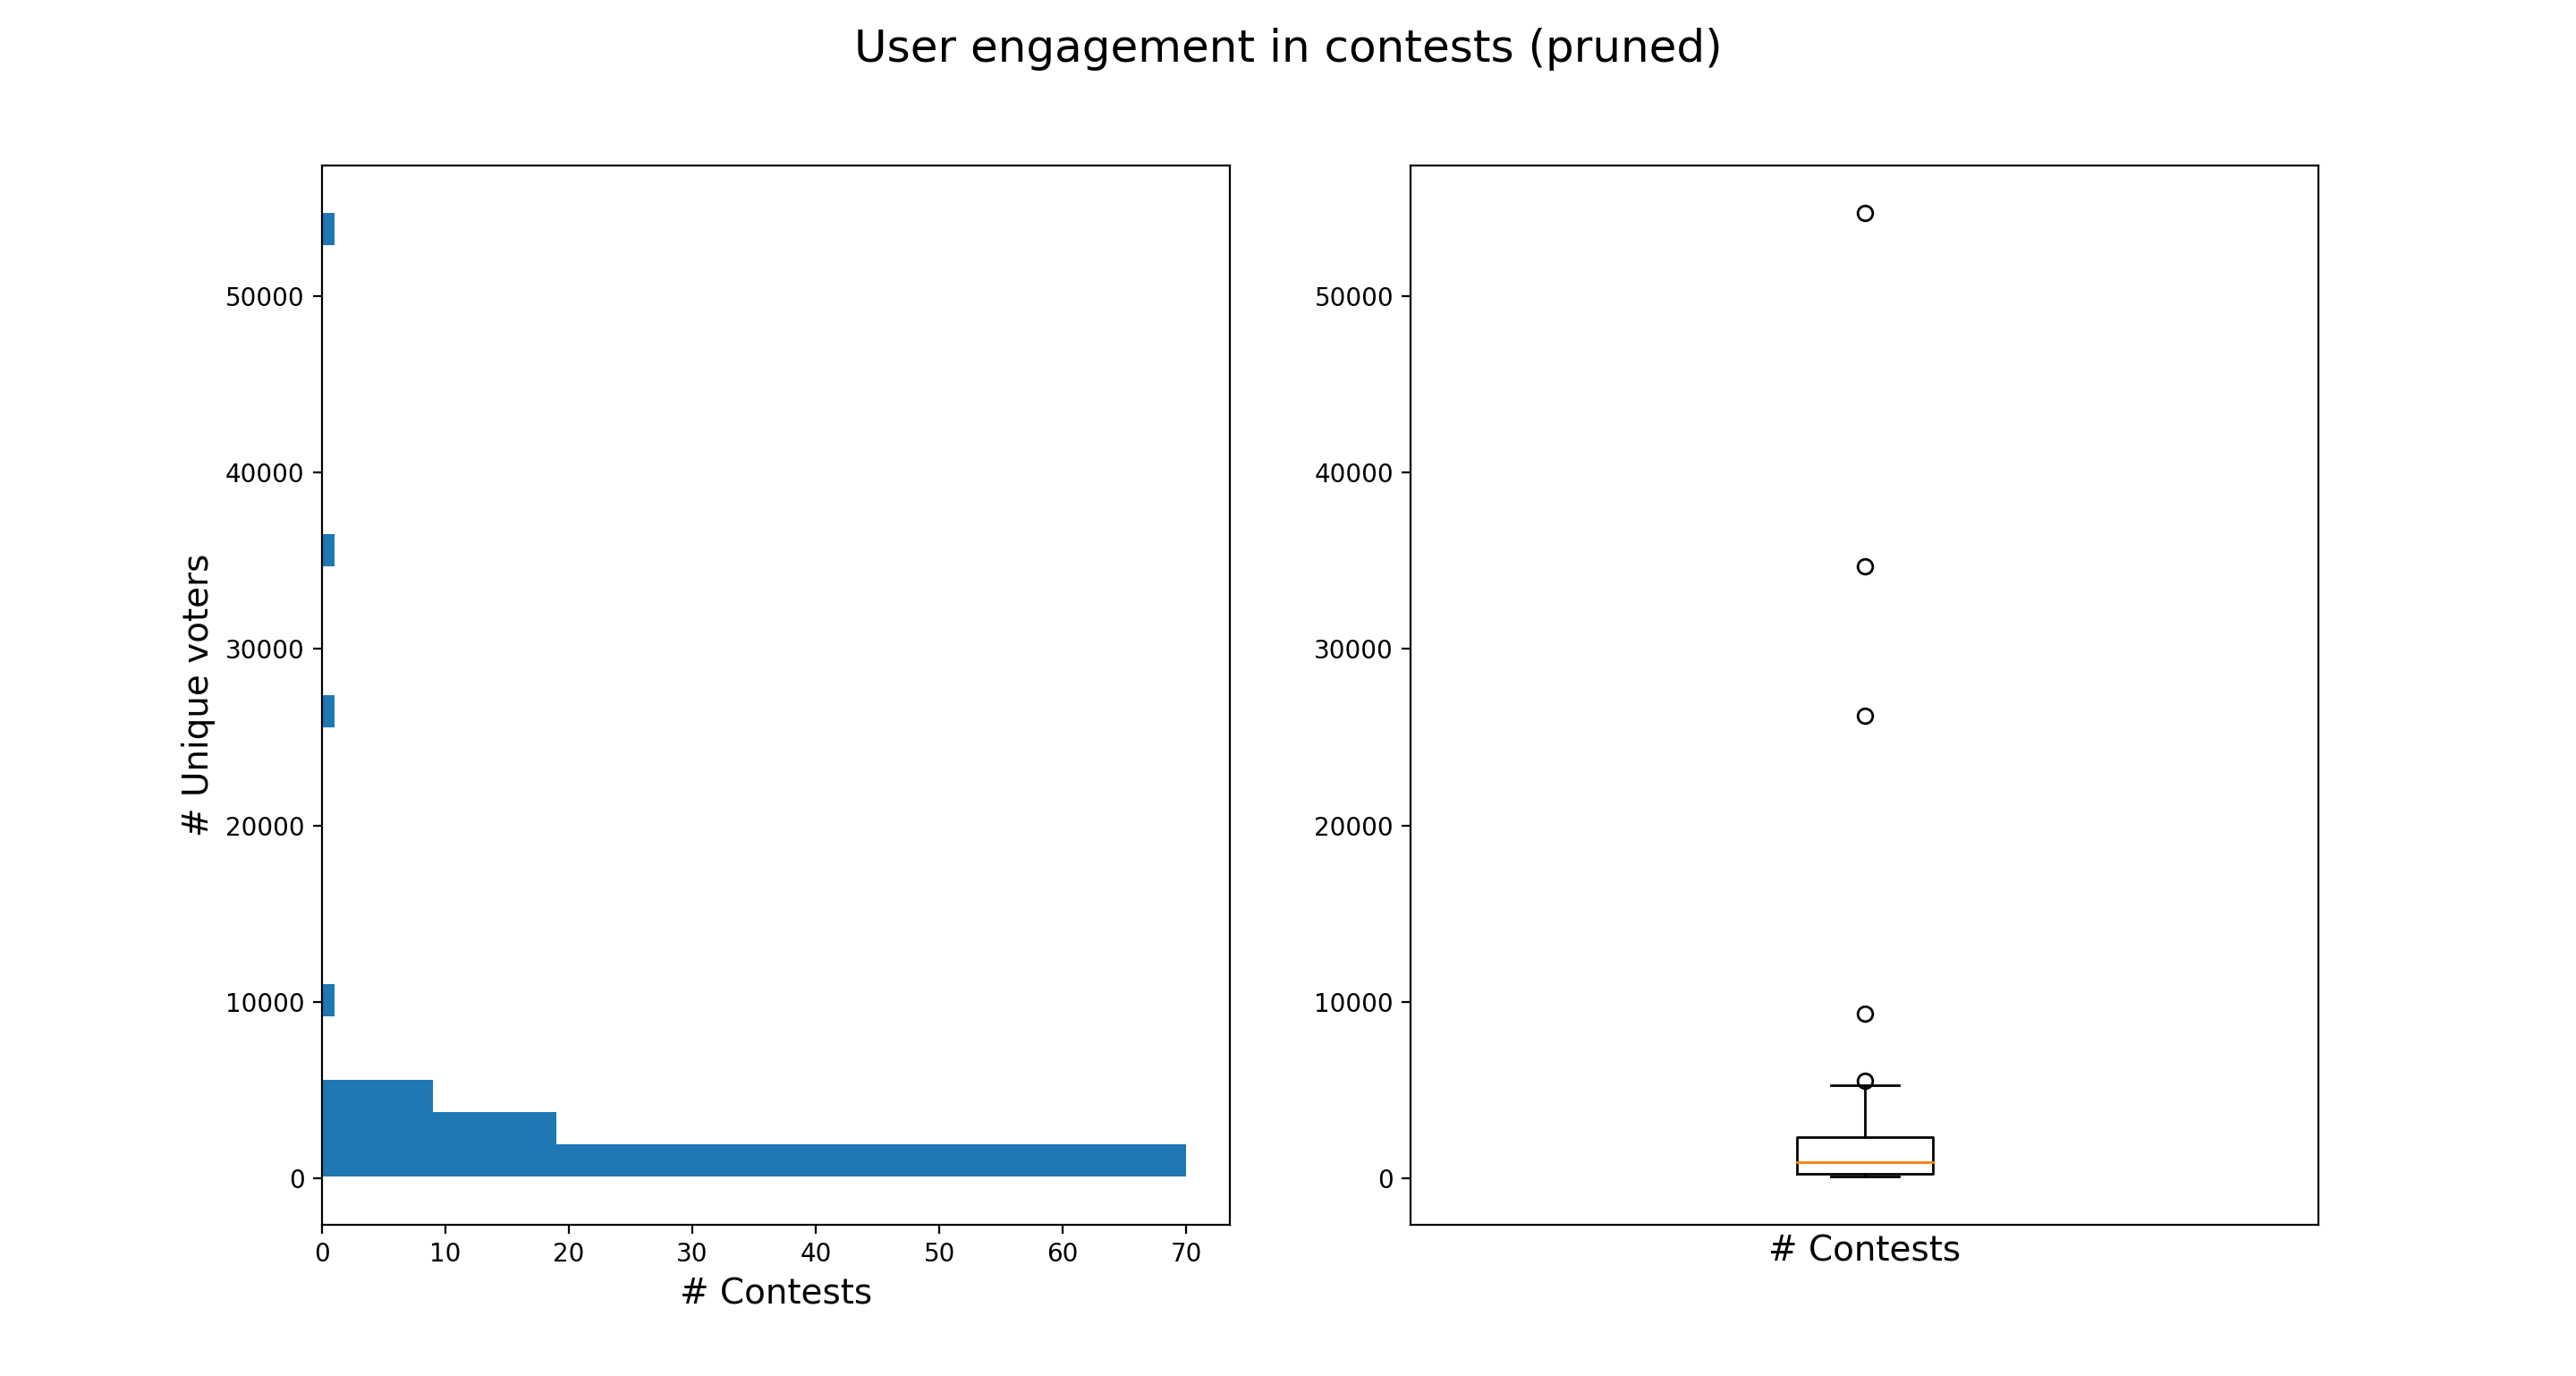
\includegraphics[width=0.8\textwidth]{Images/user_engagement_in_contests-pruned.png}
            \caption{The number of unique voters over contests after filtering out contests with less than $100$ unique voters.}
            \label{user_engagement_in_contests-pruned}
        \end{center}
    \end{figure}
    
    The six large contests are worth investigating a bit more closely. Four \footnote{\url{https://choicely.com/contest/5ca98554-0f7d-11e7-9f0c-6f102a54d68d}}\footnote{\url{https://choicely.com/contest/fb112461-9000-11e6-9e28-87ebd7a21d0d}}\footnote{\url{https://choicely.com/contest/7425566e-8c8e-11e6-b8ce-2147b021362f}}\footnote{\url{https://choicely.com/contest/164f52c7-9df8-11e7-b3c9-d1a0f88250ad}}
    out of the six large contests were beauty pageants, labeled with the categories of "beauty", "fashion" and "entertainment". The two other contests
        \footnote{\url{https://choicely.com/contest/50819173-f838-11e6-b171-b949f18a4d21}}
        \footnote{\url{https://choicely.com/contest/4257ea9c-3e21-11e7-84ec-5f5a9bcfd190}}
    are listed only in the "other" category, which is certainly a mistake. By looking at the latter two contests, it can be easily seen that they would better belong to the "entertainment" and "sports" category. In each of the contests, the contest participants were people: either sportsmen, celebrities or beauty queens/kings. It is interesting that none of the large contests have had objects, places or other intangibles as contest participants, although the platform has seen many of such participants previously. The number of participant in these contests varies between $9-40$ and their correlation coefficient does not show strong relationship either way ($R = 0.53$). 

    In the next step, let us look at the distribution of contest categories in the filtered set of contests. It can be seen from the histogram on Figure \ref{contests_over_categories}, that a considerably high number of contests ($235$) are categorized under the "other" category. After filtering out contests with only to the "other" category, it was identified that many of the sports, humor, design, beauty and fashion-related contests were indeed not labeled correctly upon creation. On top of that, many contests appear only in the "other" category (without any further categories attached), which is the default value for all contests in the platform.
    
    This observation can be explained by the fact that authors did not assign the categories for one reason or another. It can be also seen that the amount of "beauty" and "fashion" contest is considerably high compared to the other categories, which is in align with the case company's profile at the point of conducting this study. From this visualization it is also visible that the amount of "sports" contests is considerably low ($74$) knowing the company's history and customer base. 

    % number of contests in overall, by category
    % explain the findings that there were too many "other" type of contests which were fixed manually
    \begin{figure}[h] 
        \begin{center}
            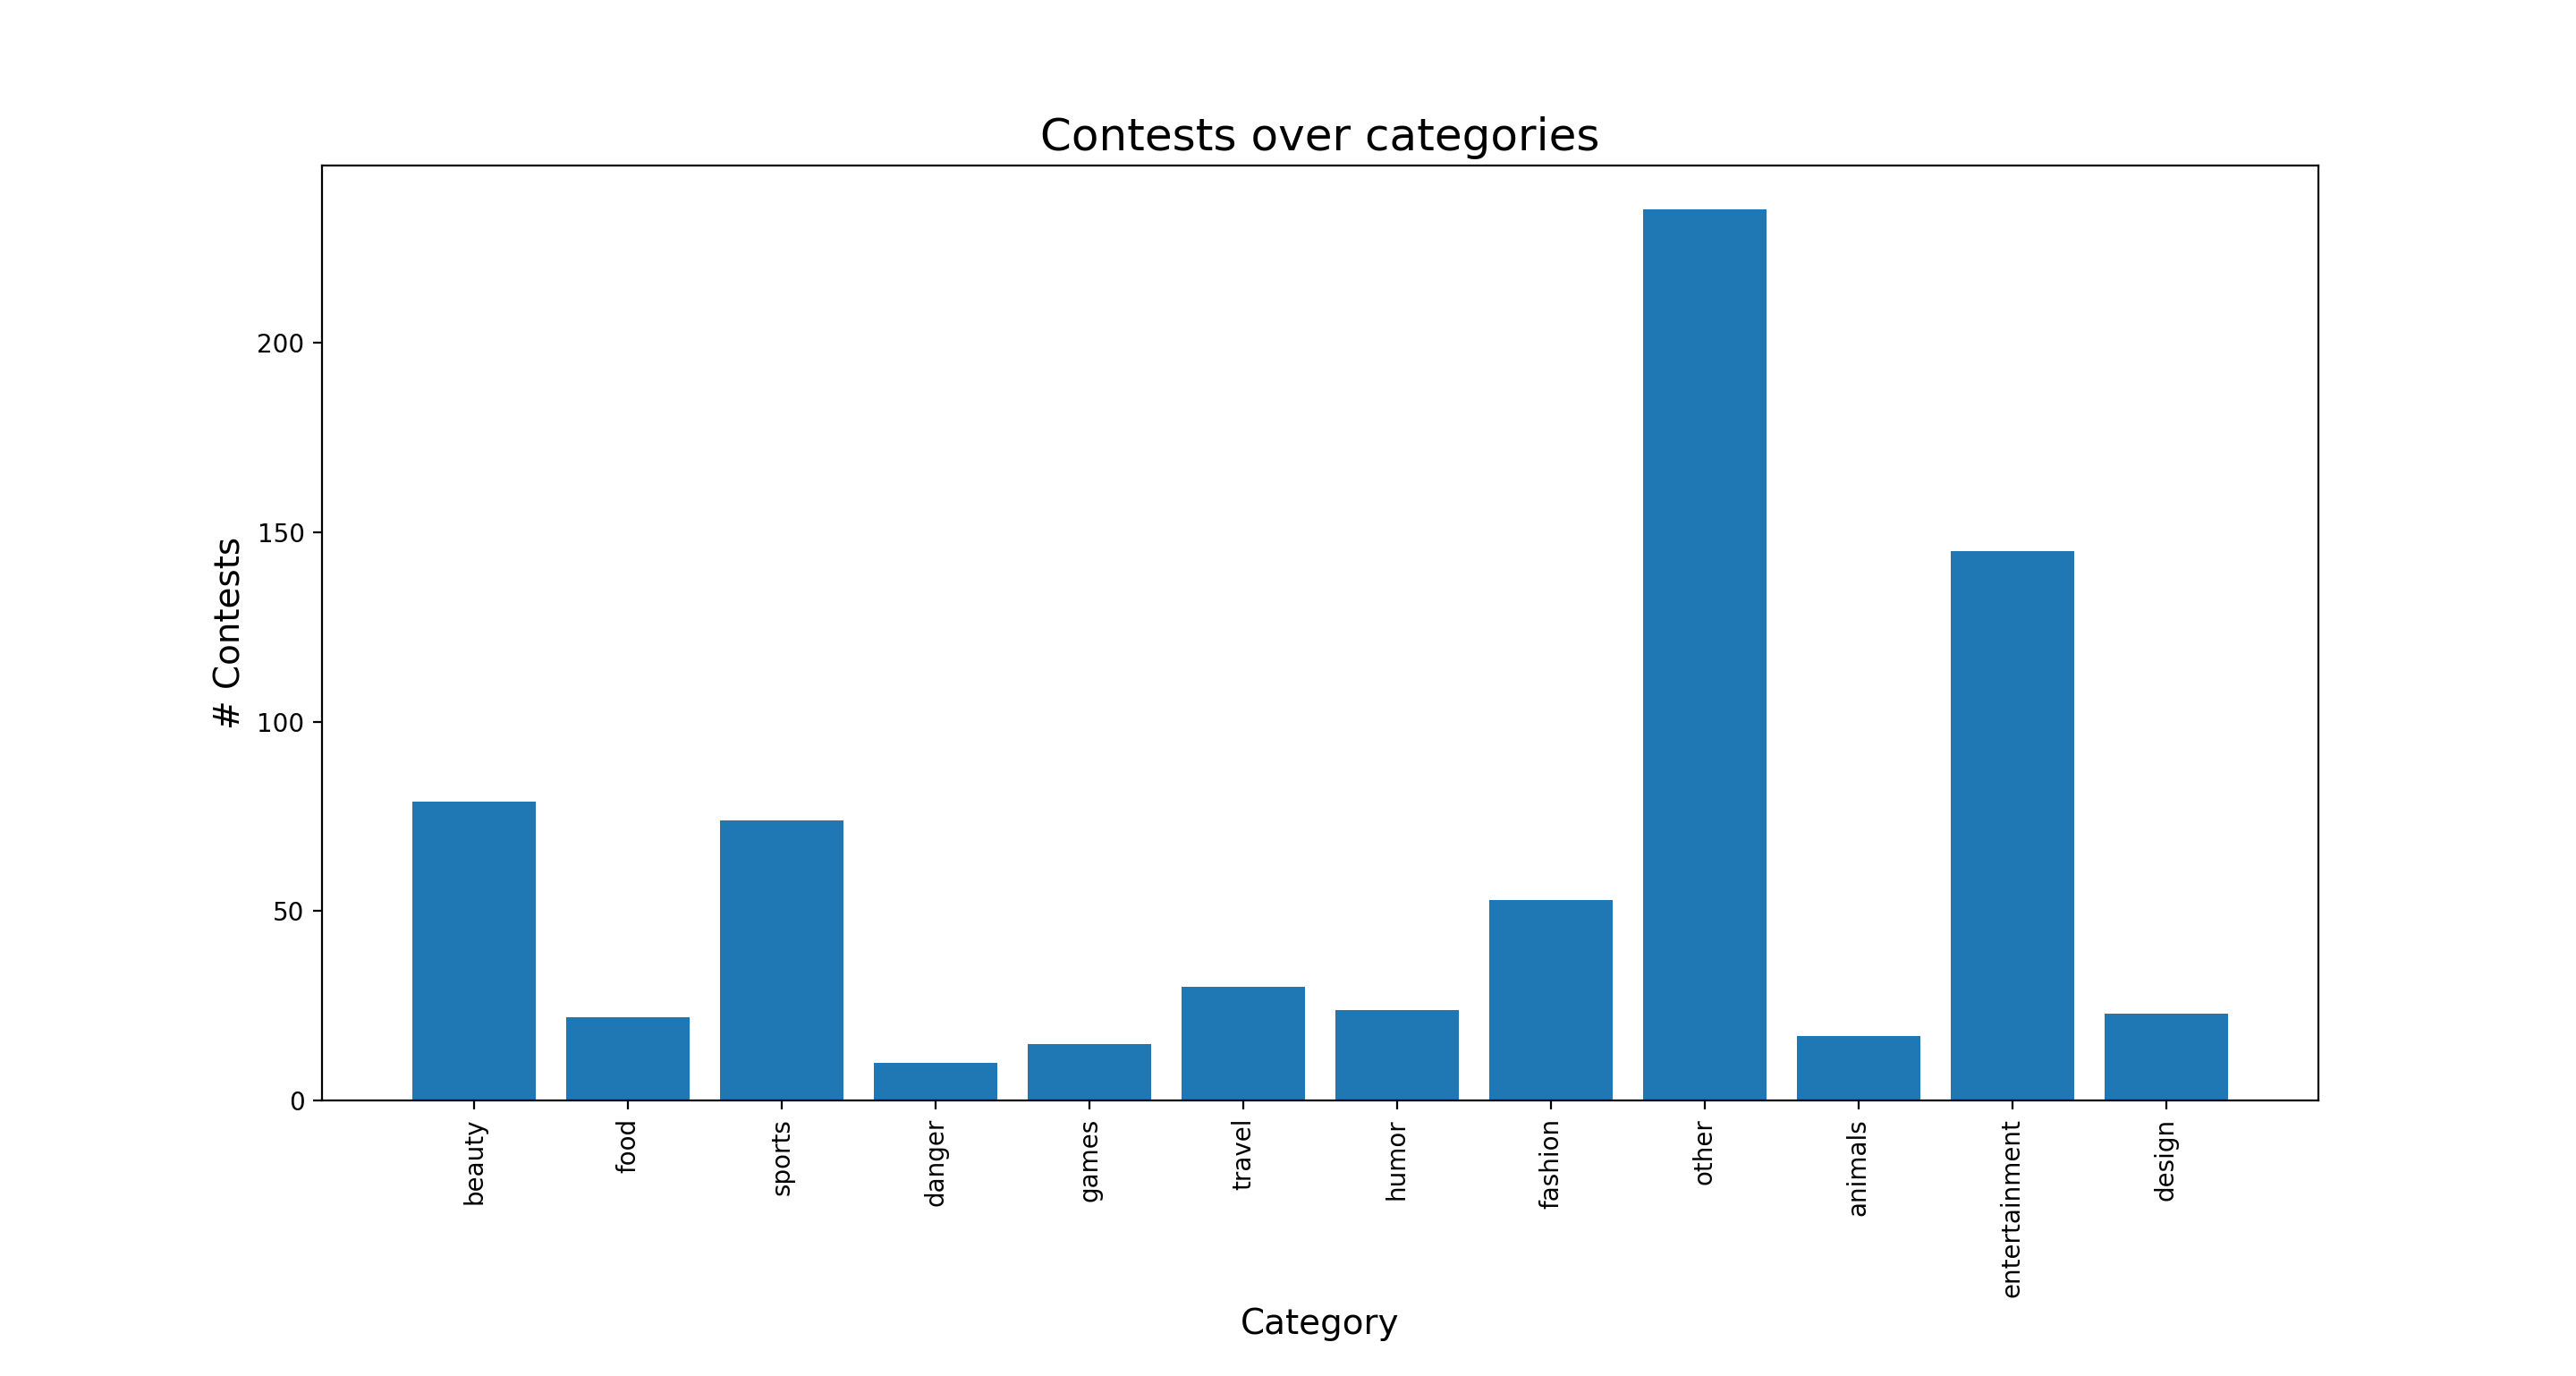
\includegraphics[width=0.8\textwidth]{Images/contests_over_categories.png}
            \caption{The number of contests in each category.}
            \label{contests_over_categories}
        \end{center}
    \end{figure}
    
    To answer the question of most engaging contest categories, the unique voters over contest categories is studied. From Table \ref{user_engagement_over_categories} it can be seen, that "entertainment" and "beauty" contests cover the majority the voters ($\approx 66.60 \%$ of the total). In these categories the mean and the median of the voters is also considerably high, which suggests the success of these categories. However, the number of contests in these categories is also higher compared to the others. Because the other categories, shuch as "food", "danger" and "games" have not seen high number of contests yet, it is difficult to say anything about their attractiveness.

    \begin{table}[]
        \centering
        \begin{adjustbox}{width=1\textwidth}
            \begin{tabular}{l|c|c|c|c|c}
                \textbf{Contest category} & \textbf{Number of contests} & \textbf{Sum of unique voters} & \textbf{Mean of unique voters} & \textbf{Median of unique voters} & \textbf{Standard deviation of unique voters} \\
                \hline
                beauty & 34 & 135866 & 3996.06 & 1482.00 & 9854.14 \\
                other & 34 & 61455 & 1807.50 & 1240.50 & 1831.40 \\
                entertainment & 30 & 161233 & 5374.43 & 1728.50 & 11772.68 \\
                sports & 24 & 15220 & 634.17 & 299.00 & 757.83 \\
                fashion & 16 & 75872 & 4742.00 & 874.00 & 12972.72 \\
                travel & 3 & 4451 & 1483.67 & 409.00 & 1719.40 \\
                humor & 2 & 1367 & 683.50 & 683.50 & 274.50 \\
                food & 1 & 767 & 767.00 & 767.00 & 0.00 \\
                danger & 1 & 958 & 958.00 & 958.00 & 0.00 \\
                games & 1 & 164 & 164.00 & 164.00 & 0.00
            \end{tabular}
        \end{adjustbox}
        \caption{The basic statistical measures of unique voters for each contest category.}
        \label{user_engagement_over_categories}
    \end{table} 

    % deriving results
    The above results contribute towards answering RQ2. The results allow to derive the following conclusions: 

    \begin{itemize}
        \item many of the contests are not labeled and hence belong only to the "other" category - fixing these labels manually could contribute towards better results,
        \item contests in the "beauty" and "entertainment" category appear to be engaging to large audiences,
        \item contests where participants are human beings appear to be attractive to users,
        \item there is no correlation between the unique voter count and the number of participants,
        \item the platform has hosted only a few contests in some of the categories and hence it is not possible to derive significant findings about the attractiveness of those contets at the moment.
    \end{itemize}

\subsection{Association analysis}
